\documentclass{article}%
\usepackage[T1]{fontenc}%
\usepackage[utf8]{inputenc}%
\usepackage{lmodern}%
\usepackage{textcomp}%
\usepackage{lastpage}%
\usepackage[head=40pt,margin=0.5in,bottom=0.6in]{geometry}%
\usepackage{graphicx}%
%
\title{\textbf{OVSC ante la CIDH pidió cese de la criminalización de la protesta pacífica}}%
\author{El Nacional Web}%
\date{04/10/2018}%
%
\begin{document}%
\normalsize%
\maketitle%
\textbf{URL: }%
http://www.el{-}nacional.com/noticias/politica/ovsc{-}ante{-}cidh{-}pidio{-}cese{-}criminalizacion{-}protesta{-}pacifica\_254342\newline%
%
\textbf{Periodico: }%
EN, %
ID: %
254342, %
Seccion: %
Política\newline%
%
\textbf{Palabras Claves: }%
Política, OEA, Crisis humanitaria\newline%
%
\textbf{Derecho: }%
5, %
Otros Derechos: %
18, %
Sub Derechos: %
\newline%
%
\textbf{EP: }%
SI\newline%
\newline%
%
\textbf{\textit{Marco Ponce, representante del Observatorio Venezolano de Conflictividad Social, aseguró que en lo que va de año se han registrado más de 8.000 protestas por violación a los derechos de los venezolanos}}%
\newline%
\newline%
%
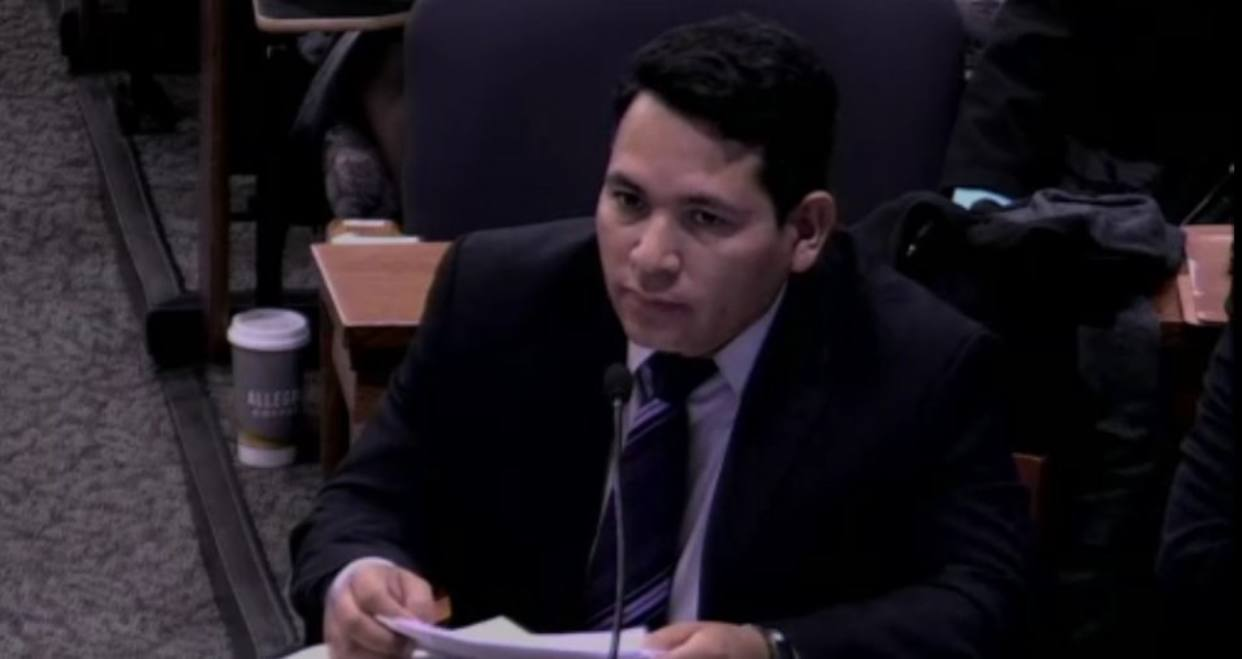
\includegraphics[width=300px]{90.jpg}%
\newline%
%
Marco Ponce, coordinador del Observatorio Venezolano de Conflictividad Social (OVCS), indicó que en Venezuela hay una emergencia humanitaria que crece diariamente como consecuencia de la hiperinflación. Aseguró que la crisis pudo ser evitada utilizando los métodos adecuados, sin embargo, el gobierno de Nicolás Maduro~no actuó a favor de un cambio.%
\newline%
%
El representante del OVCS informó, durante su intervención en la audiencia de la Comisión Interamericana de los Derechos Humanos, que los venezolanos sufren la sistemática violación de sus derechos. En el país se registraron más de 8.000 protestas en lo que va de año por falta de servicios básicos, como agua, luz y gas, y por la necesidad de mejorar la capacidad adquisitiva de los ciudadanos.%
\newline%
%
"Los que más han protestado han sido los trabajadores, vecinos y adultos mayores para exigir sus derechos. El espiral de conflicto va a seguir aumento si no se toman medidas", declaró Ponce que acotó que este año 14 manifestantes han sido asesinados.%
\newline%
%
Ponce solicitó en la audiencia el cese de la criminalización de las protestas de los ciudadanos, que a su juicio, sirve de excusa para vulnerar aún más sus derechos.%
\newline%
%
Este jueves se celebra en Colorado, Estados Unidos, una audiencia de la CIDH en la cual los representantes de distintos países debaten sobre la situación de Venezuela .Durante el encuentro los presentes han destacado los temas más resaltantes del país como la represión violenta de las constantes protestas pacíficas, la falta de alimentos y acceso a la salud y la violación de los derechos de los ciudadanos.%
\newline%
%
\end{document}